\question (华中理工大学,1999年)透明网桥通过( )学习其他网络节点
\par\fourch{检查网桥接收到的每一个数据帧的目标地址}{查询其他节点}{\textcolor{red}{检查数据帧的源地址}}{人工设置路由表}
\begin{solution}常见的网桥可分为透明网桥和源路由网桥。透明网桥由网桥自己决定路由选择,透明是指局域网上的每个站并不知道所发送的帧将经过哪几个网桥。透明网桥通过检查数据帧的源地址来建立连接。
\end{solution}
\question 如图3-20所示,为两个局域网LAN1和LAN2通过网桥1和网桥2互连后形成的网络结构。假设站A发送一个帧,但其目的地址均不在这两个网桥的地址转发表中,这样的结果会是该帧(
~)。

~
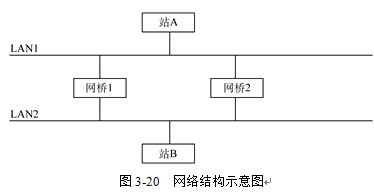
\includegraphics[width=3.88542in,height=2.03125in]{computerassets/f0166ec6a5b0627b475a77901a9b2521.jpeg}
\par\fourch{经网桥1(或网桥2)后被站B接收}{被网桥1(或网桥2)丢弃}{\textcolor{red}{在整个网络中无限次地循环下去}}{经网桥1(或网桥2)到达LAN2,再经过网桥2(或网桥1)返回LAN1后被站A吸收}
\begin{solution}当站点A发送一个目的地址均不在这两个网桥的地址转发表中的帧时,网桥1和网桥2均进行扩散传播,这样经过网桥1转发的帧将继续经过网桥2的转发,而经过网桥2转发的帧也会继续经过网桥1的转发,这样这个数据帧将在整个网络中无限制地循环下去(兜圈子)。
\end{solution}
\question (重庆大学,2005年)下面关于网桥的描述,错误的是
\par\fourch{网桥工作在数据链路层,可以对网络进行过滤和分段}{\textcolor{red}{网桥可以对不需要传递的数据进行过滤并有效地阻止广播数据}}{网桥传递所有的广播信息,因此难以避免广播风暴}{网桥与集线器相比,需要处理接收到的数据,因此增加了时延}
\begin{solution}网桥只适合于用户不多和通信量不太大的局域网,否则有时还会因传播过多的广播信息而产生网络拥塞,这就是所谓的广播风暴。
\end{solution}
